%\section{Transformation of an SDN network to an OpenFlow switch}
\section{SDN Model Abstraction}
\label{Sec:Design}

\begin{comment}
The overview of our model abstraction approach for SDN networks is shown in Figure~\ref{Fig:BigSimOverview}. Through a three-step systematic process, we are able to take 
a snapshot of an SDN network $SN$ as the input, transform the network devices in an SDN network to a single OpenFlow switch, $BS$ that preserves the forwarding logic of the original network. In this section, we elaborate the algorithmic design in each step of the model abstraction.
%We have sketched the process of how to replace a OpenFlow-switch-connected network with a single OpenFlow switch in section~\ref{Sec:MotivationalExample}.
\end{comment}

Our objective is to effectively transform a static SDN data plane configuration (i.e., a snapshot of the network state) to one ``big switch" model, which preserves the same end-to-end forwarding behavior. %In other words, if a packet originated from a host is forwarded to host in the snapshot, then the packet will be sent to the same destination by the ``big switch". 
To achieve this objective, we need to identify how every packet is processed in the snapshot, and how to correctly configure the big switch model to reflect the identical forwarding logic. In this paper, we develop a three-step model abstraction method, which is summarized as follows.

\begin{itemize}
\item \textbf{Identifying Equivalence Classes.} We partition all possible packets in the network into mutually exclusive sets (i.e., equivalence class, as formally defined in Section \ref{ec}), and the packets belongs to the same set are processed in the same way. Those sets are identified according to the matching field of \textbf{all} the OpenFlow rules on \textbf{all} the SDN switches in the original network.

\item \textbf{Creating Forwarding Graphs.} We model the forwarding behavior of each packet set using the topology information as well as the local information stored on SDN switches (e.g., port mapping, rule priorities, etc), and generate a graph-based model to represent the forwarding behavior.  
\item \textbf{Generating OpenFlow Rules of the Big Switch.} We generate the OpenFlow rules for the big switch in order to preserve the end-to-end forwarding logic. This step includes (1) constructing the port-to-host mapping, (2) generating the rules by matching the packet header of each set,  and (3) forwarding the packet to the correct output port, which is determined by traversing the forwarding graph acquired in step 2.
\end{itemize}

Our three-step approach has two assumptions. First, the controller can dynamically change the configuration of each network device, but we assume that the frequency of issuing such control messages is far less than the rate of the incoming packets. Between two configuration updates, the data plane remains unchanged. Therefore, we can exclude the SDN controller from the abstracted network model. Second, we do not consider packet header modification actions on the network device. We describe each step in details in the remainder of the section.

%We assume that both the original network and abstracted network use OpenFlow switches, and the switches compare the incoming packet to the installed rule with highest priority and then apply the action of that rule. The simplicity of OpenFlow switches enables us to analyze the behavior of the original network and synthesis the configuration of the ``big switch". 
   
\subsection{Identifying Equivalence Classes}
\label{ec}

\begin{comment}
By aggregating and slicing forwarding rules in an SDN network according to ECs, one can obtain a compact representation of the network state in terms of forwarding behavior. 
\end{comment}

We first give the definition of equivalence class (EC), and then present the data structure and algorithms to partition the packets into ECs.

\begin{definition}
An equivalence class is a set of packets that experience the identical forwarding action at \textbf{any} network device in the network. 
\label{Def:EC}
\end{definition}

\begin{comment}
%\kevin{add to one or two sentences about how to find ECs and how to aggregate ECs before the structure}
By its definition, ECs can be found by aggregate forwarding rules on different switches
and group them by the match field.
We aggregate forwarding rules using a trie structure as inspired by VeriFlow\cite{Veriflow}. 
A trie node has three child nodes, i.e., zero, one or wildcard, that represent three possible values for performing a bit-to-bit rule matching.
The entire tree is composited by several sub-tries, each representing one packet header field. For example, consider the tree-topology network in Section \ref{Sec:MotivatingExample}, the trie only contains one sub-trie representing the $NW\_DST$ header field (i.e., the network destination address). Note that an EC can be defined by multiple fields. For example, we can also match the source address of the packet (e.g., $NW\_SRC$) as well as the service type of the traffic ($TCP\_SRC$). The resulting trie now has three sub-tries.
%Here we give solutions to two problems that VeriFlow neglected.
\end{comment}

Each packet is uniquely identified by its header field values, which are matched against the forwarding rules in the OpenFlow switches to determine the appropriate action. Since the matching fields of the OpenFlow rules typically contain the wildcard suffix (e.g., longest prefix match of IP source/destination addresses), a group of packets with consecutive header values are often processed by the same rule. We use a trie structure, originally proposed by VeriFlow \cite{Veriflow}, to maintain the matching fields of all the OpenFlow rules in the network. The trie is composed of several sub-tries, and each sub-trie stands for a matching field (e.g., source/destination MAC address/IP address/port, etc.). Each node in sub-trie presents one bit in the corresponding matching field, and each node has three edges to the next node (i.e., next bit in the  matching field). The edges represent three possible bit-to-bit rule matching conditions: zero, one, or wildcard (i.e., don't care). The rule metadata are stored in the corresponding leaf node, including the rule's location (switch\#), action (forwarding to an out port or dropping the packet), priority, etc. 

Having all the OpenFlow rules inserted in the aforementioned trie structure, we perform the following three steps to identify the equivalence classes in the network. (1) We traverse the trie to obtain the consecutive header values for each rule. (2) After having a collection of header value intervals, which are denoted by the starting and end values, we develop an algorithm to split the existing intervals into smaller and non-overlapping intervals. Each non-overlapping interval identifies the packets belonging to an equivalence class. (3) We merge certain equivalence classes in order to reduce the time and space complexity for the forwarding graph generation (Section \ref{Sec:Generating Forwarding Graphs}) and the big switch rule generation (Section \ref{sec:thirdstep}). The details of second and third steps for EC identification are presented as follows.

\if 0
\begin{figure}[t]
\centering
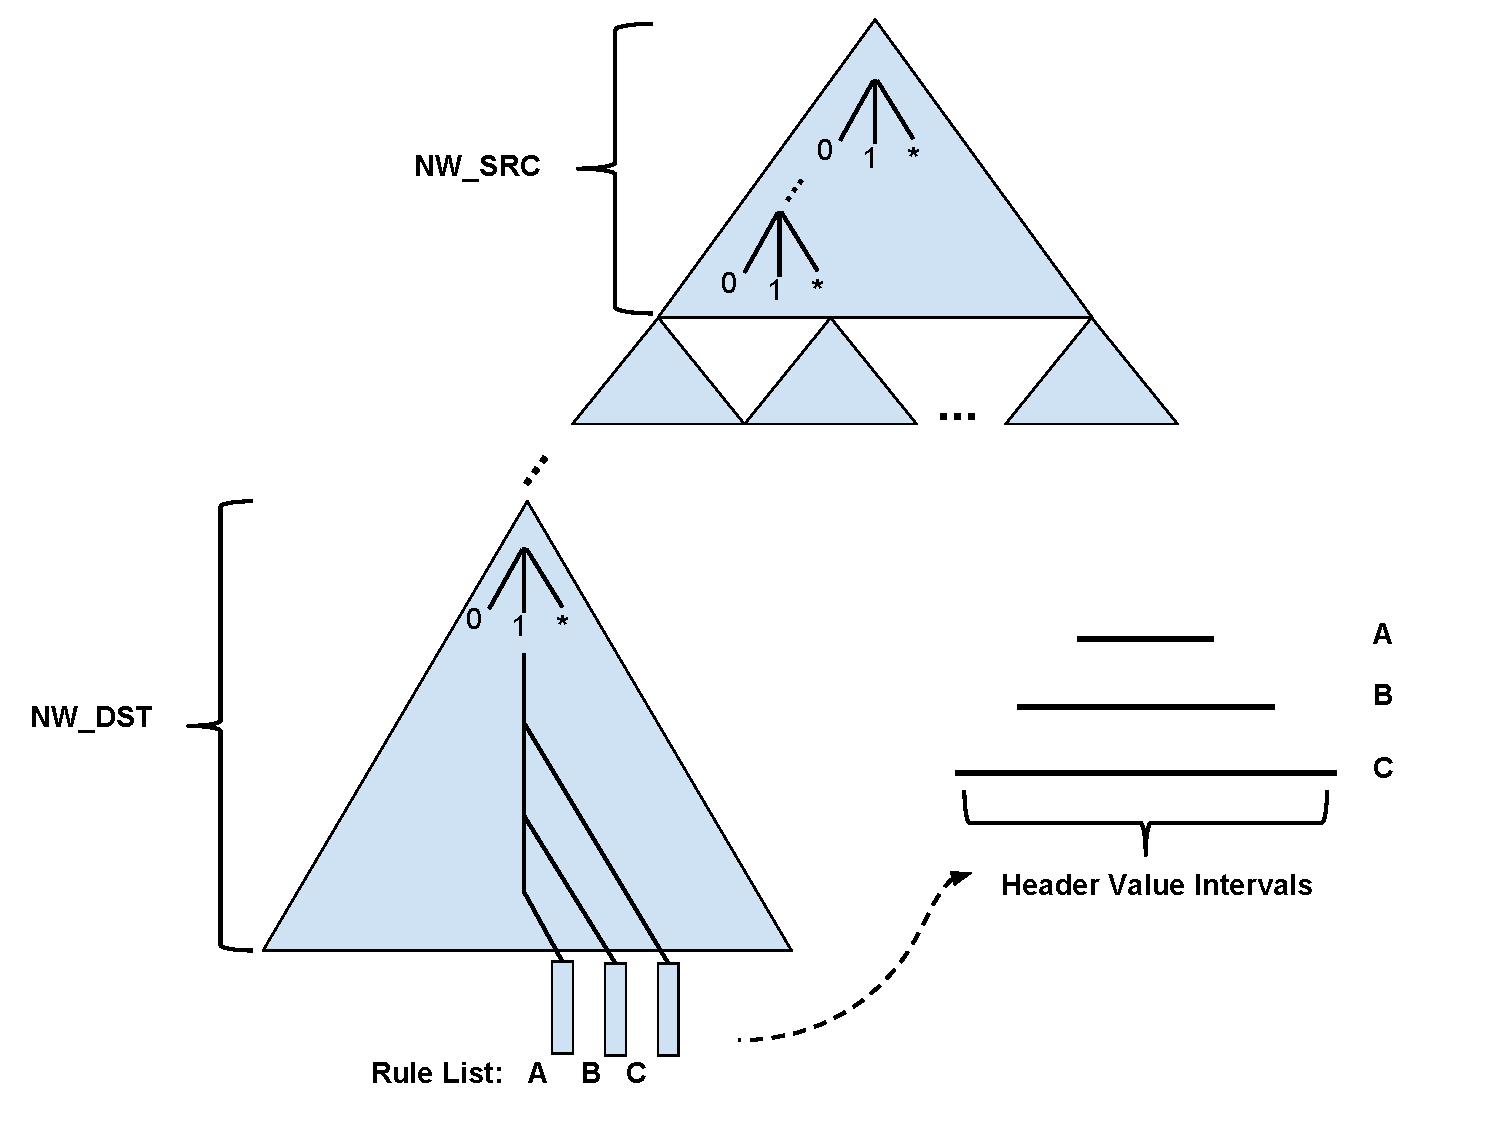
\includegraphics[scale=.35]{figures/trie.pdf}
\caption{A trie data structure to maintain header values.}
\label{Fig:Trie}
\end{figure}
\fi 

\subsubsection{Splitting Overlapping Intervals}
% Xin: I changed all the "ranges" into "intervals" or "header intervals", since the term "range" has a specific meaning in maths.
By traversing from the root node to all leaf nodes, we obtain a set of packets header intervals that match all the rules along the traversal. Each interval is represented by a pair of starting and ending values as $A, B$ and $C$ as shown in Figure~\ref{Fig:DisjointECsAsInterval}. We split this set of intervals, $I$, to a list of non-overlapping intervals, each of which forms an EC. %An example is shown in the upper part of Figure~\ref{Fig:DisjointECsAsInterval}. 
We develop Algorithm~\ref{Alg:GenDisjointECs} to generate a set of disjoint intervals, and show that the generation can be accomplished in $O(N \times M\log M)$ time,
where $M$ is the number of intervals in $I$, and $N$ is the number of header bits.
% as follows\cite{SplitDisjointInterval}.
%Not algorithmic described in\cite{Veriflow},

First, we place $I$ into an array $A$ of $2M$ elements. Each element is either a starting point or an end point of an interval. %Note that equal values with same flag are reduced to an single element.
%Before iterating $A$, we sort it, breaking the tie by putting start point before end point.
We visit each point in a sorted order, and maintain the difference $d$ between the number of visited starting points and the number of visited end points.
\begin{itemize}
\item If the current element $x \in S$ and $d > 0$,
        we end the previous interval with the ending value $x - 1$;
        Start a new interval with a starting value $x$
        (line~\ref{Alg:LineEndStart1}-\ref{Alg:LineEndStart2}).
\item If the current element $x \in E$, we end the previous interval with the ending value $x$.
        (line~\ref{Alg:LineEndEnd}).
\item In either case, we update the potential new interval's starting value \textit{prev}
        (line~\ref{Alg:LineNewPrev1} and \ref{Alg:LineNewPrev2}).
\end{itemize}
\kevin{Please define $S$ and $E$, and ``end an interval" or "start an interval" does not sound right to me, usually we start/end an action.}

Updating the network forwarding rules will change the EC set.
By maintaining the rules in a trie, we can efficiently update ECs in an incremental way. An insertion of a new rule requires us to do a depth first traversal. This process automatically narrows down the set of affected rules by ignoring those non-overlapping branches with the new rule.
The output is the set of the affected intervals, and we can run Algorithm~\ref{Alg:GenDisjointECs} to only update those affected ECs.

\begin{figure}[t]
\centering
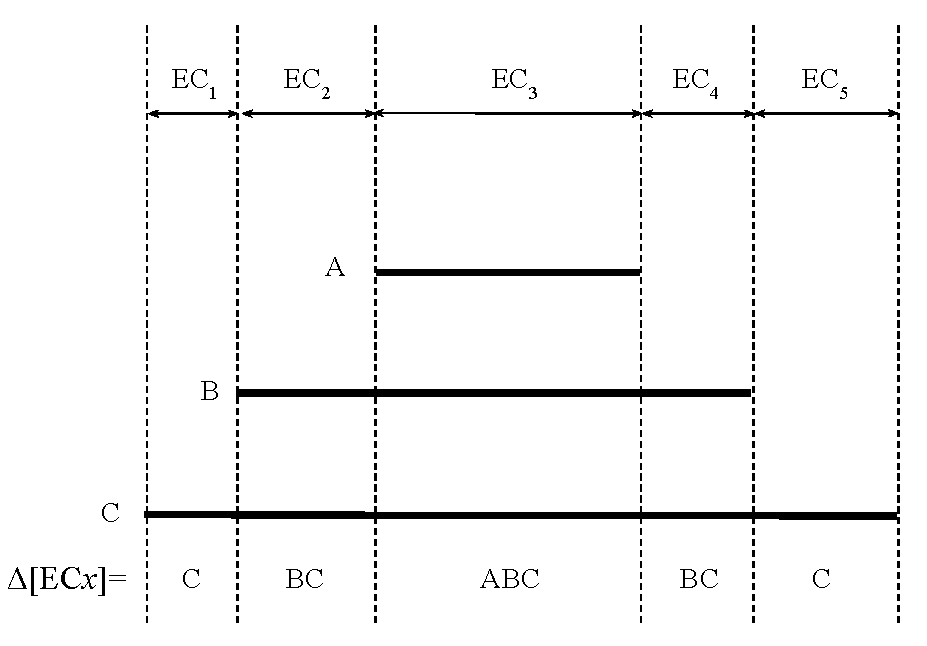
\includegraphics[scale=.52]{figures/DisjointECs.pdf}
\caption{A set of packets are identified by an interval of packet header values.
        Five equivalence classes, $EC_1$ to $EC_5$, can be obtained via splitting three intervals A, B and C.
        Finding $\Delta[EC_x]$ (i.e., the rules that intersect with $EC_x$) is instrumental for
        merging ECs, as shown in the bottom of the figure.}
\label{Fig:DisjointECsAsInterval}
\end{figure}

\begin{algorithm}[t]
\DontPrintSemicolon
\KwData{$I = $ a set of packet header intervals from the leaves of the trie}
\KwResult{$EC = $ a set of equivalence classes as disjoint intervals} \kevin{$EC$ has special meaning as equivalence class. Please use another symbol.}
$cnt \gets 0$\;
$S = $ \{starting points of $\forall i \in I\}$, $E = $ \{end points of $\forall i \in I\}$\;
$A \gets Sort(S \bigcup E)$ in a non-decreasing order\;
$EC \gets \emptyset$\;
\ForEach {$x \in A$} {
        \uIf {$x \in S$} {
                \If {$cnt \neq 0$} {\label{Alg:LineEndStart1} 
                        $EC \gets EC \text{ }\bigcup \text{} [prev, x-1]$\;
                }\label{Alg:LineEndStart2} 
                $prev \gets x$\;\label{Alg:LineNewPrev1}
                $cnt \gets cnt + 1$\;
        }
        \Else ($x \in E$) {
                $EC \gets EC \text{ } \bigcup \text{ } [prev, x]$\;\label{Alg:LineEndEnd}
                $prev \gets x + 1$\;\label{Alg:LineNewPrev2}
                $cnt \gets cnt - 1$\;
        }
}
\caption{Splitting Overlapping Intervals}
\label{Alg:GenDisjointECs}
\end{algorithm}

\subsubsection{Combining Equivalence Classes}
We can further union certain ECs obtained from Algorithm~\ref{Alg:GenDisjointECs}, if they essentially represent the identical packet forwarding behavior (see the definition of ECs). For example, $EC_2$ and $EC_4$ in Figure~\ref{Fig:DisjointECsAsInterval} can be combined as one EC, since the packets in both ECs experience the same set of forwarding rules in the network. %To generate the correct set of rules on the new ``big switch", we only need to model the forwarding behavior of either one of the ECs. In other words, for any two ECs $\alpha$ and $\beta$, we have:

\begin{lemma}
If packets in EC $\alpha$ and EC $\beta$ experience the same forwarding actions on all network devices, then $\alpha \cup \beta$ is also an EC.
\label{Lemma:MergeFG}
\end{lemma}
Combining two EC into a big one reduce the running time in the next two phases, i.e., generating forwarding graph and populating final OpenFlow rules. The number of the resulting forwarding rules in the ``big switch" can also be reduced. We present the following lemma to identify whether two ECs can be unioned.

\begin{lemma}
EC $\alpha$ and EC $\beta$ can be unioned into one EC, if both packet header values are covered by the same set of rules in the network.
\label{Lemma:MergeEC}
\end{lemma}
%According to Lemma~\ref{Lemma:MergeEC}, 
For example, both $EC_2$ and $EC_4$ are covered by interval $B$ and $C$ in Figure~\ref{Fig:DisjointECsAsInterval}, and therefore, we can treat them as one EC. The explanation is illustrated below.

First, we define a function $\Delta(x)$ that maps an EC $x$ to a set of forwarding rules, whose matching fields cover the header values of all the packets in $x$. Assume $\Delta(\alpha) = \Delta(\beta)$, and let $\delta \in \Delta(\alpha)$ be the rule on a network device $d$ with the highest priority. 
If no such $\delta$ exists, packets from both $\alpha$ and $\beta$ are dropped on $d$.
Otherwise, packets in both $\alpha$ and $\beta$ match the rule $\delta$ and are processed with the same action specified in $\delta$.
Note that in another device $d'$, the highest priority rule that covers both $\alpha$
and $\beta$ may be different, i.e., $\delta' \neq \delta$.
However, as long as $\delta$ is unique at a given $d$, the forwarding behavior at $d$ for both $\alpha$ and $\beta$ are always identical.

Given an EC, we can efficiently calculate $\Delta(\alpha)$ using two data structures: an array of pointers and a central interval tree.
Each of them is responsible for one of the two cases specified in \cite{FindIntersectionWiki}.
\begin{itemize}
\item Case 1: A rule $\delta$ overlaps with an EC $\alpha$ with its starting and/or end point in $\alpha$.
        We can reuse the sorted array $A$ in Algorithm~\ref{Alg:GenDisjointECs}.
        We augment each value, either a starting point or an end point of an interval in $A$ with a pointer to the corresponding rule.
        By doing a binary search, we can find the minimum and maximum values in $A$,
        which bound the interval of $\alpha$.
        %All intervals that overlap with $\alpha$ must be between the minima and maxima,
       Therefore, we can ignore two types of rules: the ones with end points smaller than the minima and the ones with starting point larger than the maxima.
        We then perform a linear search in the new set of rules, and check one-by-one whether the interval overlaps with $\alpha$.
        The total time complexity for both the linear search and the binary search are $O(\log M + K)$,
        where $K$ is the number of reported intervals in $\Delta(\alpha)$.
        
\item Case 2: Rule $\delta$ covers $\alpha$ entirely. We can build
        a central interval tree\cite{ComputationalGeometryBook} with all the available intervals.
        We pick a random value $x \in \alpha$ and query the central interval tree for
        all the ranges that intersect with $x$, which can be done in $O(\log M + K)$ time. It takes $O(M log M)$ time to build the central interval tree.
        Since the central interval tree supports efficient incremental operations (i.e., insertion and deletion), our design also supports dynamic changes of the rule set.
\end{itemize}

Using the interval tree and the ordered list, for each EC $\alpha$,
we calculate $\Delta(\alpha)$ by mapping each rule $\delta \in \Delta(\alpha)$ to a unique binary ID $c_\delta$ of length $\log_2 M$.
We can encode $\Delta(\alpha)$ to a string of $c_\delta$s, starting with small IDs.
This string of unique IDs, named $C_\alpha$, has a $M\log_2 M$ upper bound in length.
We then use a hash table $H$ to combined the ECs by hashing each EC $x$ to $C_x$.
The minimal size of ECs is the number of unique keys in $H$.
Note that in the subsequent algorithmic designs, iterating through all ECs refers to iterating through the first ECs in each set $H[key]$.%, $\forall key \in H$.

\subsection{Generating Forwarding Graphs}
\label{Sec:Generating Forwarding Graphs}

In the second step, we compute a forwarding graph for each EC, and then effectively reduce the size of the forwarding graph to improve efficiency for the third step. 

First, we define a function $FG(\alpha)$ that maps an EC $\alpha$ to a corresponding forwarding graph. A forwarding graph is a directed graph that represents how packets belonging to the same EC are processed by the network. A node $u$ in the forwarding graph is a networking device, and an edge $(u, v)$ in the graph means that device $u$ forwards the packets to device $v$ in the network. 
A forwarding graph not only concatenates the forwarding behavior for each EC, but also visualizes the data flow of the EC in the network. 
%For a fixed EC $x$, we connect the network devices that have rules for $x$ with directed edges that point to the next hop, which is determined by the action field of the rule.
Since our objective is to abstract the network forwarding logic into a big switch, our end-to-end modeling focuses on the sources and sinks of the graph. 
Figure~\ref{Fig:ForwardingGraphECX} depicts the generalized forwarding graph $FG(x)$ for EC $x$. 
 
%Here we discuss two specific issues in the forwarding graph generation: where to start the traversal according to our needs and what we can achieve at the end of the traversal.

\begin{figure*}[t]
\centering
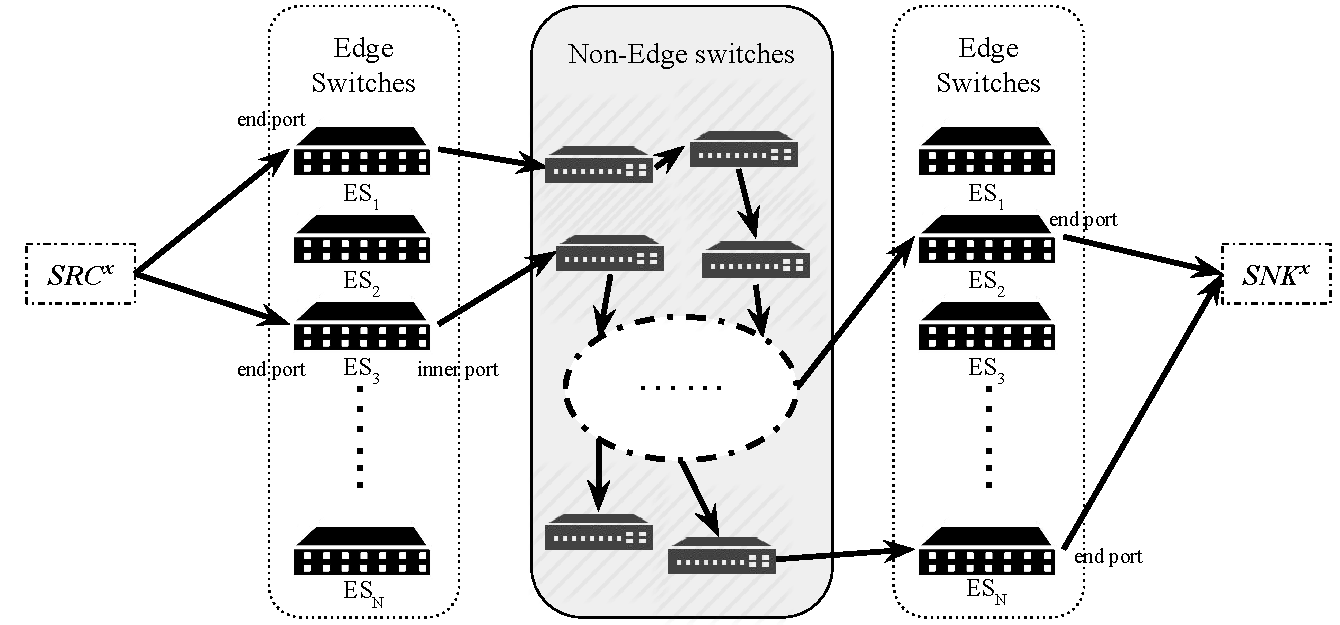
\includegraphics[scale=.75]{figures/ForwardingGraph.pdf}
\caption{Modeling a Forwarding Graph of an Equivalence Class}
\label{Fig:ForwardingGraphECX}
\end{figure*}

\subsubsection{Network Traversal for Forwarding Graph Generation}

We develop a forwarding graph generation algorithm as shown in Algorithm~\ref{Alg:GenForwardingGraph}.
The notations are defined as follows.
$FG(x)$ denotes the forwarding graph for a particular equivalence class x.
A \textit{edge switch} is defined as a switch that has at least one link to a node outside $SN$. \kevin{$SN$ first appeared here, need definition.}
A \textit{non-edge switch} is defined as a switch with all the connected node inside $SN$.
The forwarding behavior of the non-edge switches are not considered in the big switch model abstraction.
Let $src$ and $snk$ denote the source and sink nodes of the forwarding path for an EC.
Note that all $src$ in $FG(x)$ are edge switches,
and $snk$ in $FG(x)$ can be either edge switches or non-edge switches.
Let $curr$ denote the current traversed node in the network.
We add a super-source node, $SRC^x$, and a super-sink node, $SNK^x$, as the boundaries of $FG(x)$.

Algorithm~\ref{Alg:GenForwardingGraph} is designed to generate $FG(x)$.
We start the process from each $src$ that connects to $SRC^x$,
and then traverse EC $x$'s forwarding graph using a depth-first-based search and
follow the action specified in the forwarding rule with the highest priority for EC $x$ at each node along the traversal. 

%(2) the inner graph may contain both edge and internal switches.
%Source node $src$ and its out-going edge represent an edge switch $sw$ that forwards EC $x$ \textbf{coming from} port $p$; it can be described by $(sw, p)$ pair. Sink node $snk$ represent the end of the forwarding $sw$, which is also denoted by $(sw, p)$, where $p$ is either the port number specified by the action field or \texttt{NULL} if there is no rule for $x$ on $sw$.
%We denote the set of source nodes as $SRC(x)$, the set of sink nodes as $SNK(x)$.

We distinguish two kinds of port on an edge switch:
\begin{itemize}
\item \textit{end port} that connects to a node that is either the forwarding end point or outside the target network;
\item \textit{inner port} that connects to a node inside the target network.
\end{itemize}

We add an edge from $SRC^x$ to a $src$, if the source node has a forwarding rule $r$ that matches EC $x$, or the $IN\_PORT$ field of rule $r$ on the source node is an end port. 
Otherwise, we do not initiate a traverse (see line~\ref{Alg:LineStartDFS1} to~\ref{Alg:LineStartDFS2} in Algorithm~\ref{Alg:GenForwardingGraph}).
Correspondingly, we add an edge from a $snk$ to the super sink $SNK^x$, if the following two conditions are satisfied:
\begin{enumerate}
\item the sink node is an edge switch in the network;
\item the $OUT\_PORT$ field determined by the rule's action on the sink node is an end port.
\end{enumerate}

\begin{algorithm}[h]
\DontPrintSemicolon
\KwIn{$nodes = $ Switches containing rules for EC $x$ \newline
        $topo = $ Network topology}
\KwResult{Forwarding graph $FG(x)$ for EC $x$}
\SetKwProg{Fn}{Function}{}{\KwRet}
\SetKwFunction{Traverse}{traverse}
\SetKwFunction{GenRule}{generate\_rules}
\Fn{\Traverse{$curr$, $src$, $snk$}} {
        \uIf {$curr$ \upshape is \textbf{NOT} visited} {
                $r \gets$ \textbf{highest-priority} rule on $curr$ that processes EC $x$\;
                \If {r \upshape is NULL or $r.action$ is DROP} {\label{Alg:LineDropPath1}
                        $snk \gets$ ($curr$, NULL)\;
                        \GenRule{$x, src, snk$}\;
                        \KwRet\;
                }\label{Alg:LineDropPath2}
                $next \gets topo[curr][r.action.outport]$\;
                \If {next $\not\in$ nodes} {\label{Alg:LineForwardPath1}
                        $snk \gets$ ($curr$, $r.action.outport$)\;
                        \GenRule{$x, curr, src, snk$}\;
                        \KwRet\;
                }\label{Alg:LineForwardPath2}
                mark $curr$ as visited\;
                \Traverse{$next, src, snk$}\;
        }
        \Else {
                report forwarding loop\;\label{Alg:LineLoopPath}
        }
}\;
\ForEach{$n \in$ \upshape neighbors of $SRC^x$} {\label{Alg:LineStartDFS1}
        \If {\upshape $n$ is \textbf{NOT} visited} {
                $inport \gets$ input port number from $SRC^x$ to $n$\;
                \Traverse{$n$, $src=$\upshape($n$, $inport$), $snk=$NULL}\;
        }
}\label{Alg:LineStartDFS2}
\caption{Generating a Forwarding Graph for EC $x$\label{Alg:GenForwardingGraph}}
\end{algorithm}


\subsubsection{Network Traversal Outcomes}
After running Algorithm~\ref{Alg:GenForwardingGraph}, we can discover three kinds of ``path" in $FG(x)$ that are useful for the forwarding rule generation process for the big switch model, i.e., the third step of our model abstraction process (see Section \ref{sec:thirdstep}). 

\begin{itemize}
\item \textbf{Forwarding path} (line~\ref{Alg:LineForwardPath1}-\ref{Alg:LineForwardPath2}).
        The path from the super source node to the super sink node.
        This is a normal forwarding path for packets in EC $x$.
        
\item \textbf{Dropping packets in the network} (line~\ref{Alg:LineDropPath1}-\ref{Alg:LineDropPath2}).
        The path ends at a device inside the network, and fails to reach the super sink node. This indicates that the packets in EC $x$ are dropped inside the network.
        
\item \textbf{Forwarding loop} (line~\ref{Alg:LineLoopPath}).
        There is a directed cycle in the graph. One can simulate a forwarding loop in the network by (1) adding a rule in the big switch to drop the looping packets; or (2) dynamically monitoring the volume of the looping packets and adjusting the delay of looping packets and other packets sharing the communication path. We choose the first method since the model abstraction in the paper is focus on the forwarding logic equivalence, and will leave the second method as future work when investigating end-to-end performance equivalence. 
        %This behavior can be emulated in the semantic of \textbf{performance equivalence}, but not by \textbf{logical equivalence} studied in this paper.        
        %(1) recording the volume of the looping packets;
        %(2) increasing the delay of other packets on the basis of the amount of looping packets
\end{itemize}

\subsection{Populating Flow Tables on the Big Switch Model}\label{sec:thirdstep}

\begin{algorithm}[htbp]
\DontPrintSemicolon
\KwData{$PortMap$, which maps a $port$ on $sw$ to a $port$ on the big switch\newline
        $global\_port$, for port number assignment, and is initialized to 0}
\KwResult{A new rule $r$ to install on the big switch}
\SetKwProg{Fn}{Function}{}{\KwRet}
\SetKwFunction{GenRule}{generate\_rules}
\Fn{\GenRule{$x, src, dst$}} {
        $r.match \gets x$\;\label{Alg:LineMatch}
        \If {src.port $\not\in$ PortMap[src.sw]} {
                $PortMap[src.sw][src.port] \gets global\_port++$\;
        }
        $r.inport = PortMap[src.sw][src.port]$\;\label{Alg:LineInport}
        \uIf {dst.port \upshape is NULL} {
                $r.action \gets $ drop\_action\;\label{Alg:LineGenDropRule}
        }
        \Else {
                \If {dst.port $\not\in$ PortMap[dst.sw]} {\label{Alg:LineGenForwardRule1}
                        $PortMap[dst.sw][dst.port] \gets global\_port++$\;
                }
                $r.action \gets $ forward\_action\;
                $r.action.outport \gets PortMap[dst.sw][dst.port]$\;\label{Alg:LineGenForwardRule2}
                
        }
}
\caption{Generating Forwarding Rules for EC $x$ on the Big Switch Model \label{Alg:GenAllRules}}
\end{algorithm}

We develop an algorithm to generate OpenFlow rules on the big switch to abstract the forwarding behavior (see Algorithm~\ref{Alg:GenAllRules}).
%by calling \texttt{generate\_rules}, as described in Algorithm~\ref{Alg:GenAllRules}.
We maintain a hash table $PortMap$ to map the end ports of the edge switches to the ports of the big switch.
This table is configured using the $global\_port$ variable during the rule generation procedure. 
Algorithm~\ref{Alg:GenAllRules} generates the mandatory fields in an OpenFlow rule:
\begin{itemize}
\item The $MATCH$ field is given by the EC $x$, i.e., the range of matching packets header (line \ref{Alg:LineMatch});
\item The $IN\_PORT$ field is the mapped port number of $src.port$ (line~\ref{Alg:LineInport});
\item Depending on the $dst$ port, we generate either a packet drop action (line~\ref{Alg:LineGenDropRule}) or a packet forwarding action with the appropriate mapped port number of $dst.port$ (line~\ref{Alg:LineGenForwardRule1}-\ref{Alg:LineGenForwardRule2}).
\end{itemize}


